\clearpage{}
\section{Define software requirements. Discuss means and stakeholders of
requirements elicitation. Describe the different types of requirements and
their desired characteristics. Explain and distinguish the nature of
requirements definition and specification documents.}

\subsection{Software requirements}

A requirement is an expression of desired behaviour. A requirement deals with objects or
entities, the states they can be in, and the functions that are performed to change states or
object characteristics. We are looking for requirements that identify key entities, limit
entities or define relationships among entities. \newline

Focus on the customer needs, NOT on the solution or implementa1on $\rightarrow$ what behaviour is
needed, NOT how that behaviour will be realized. \newline

\subsubsection{The requirements process}

\begin{figure}[!ht]
    \centering
    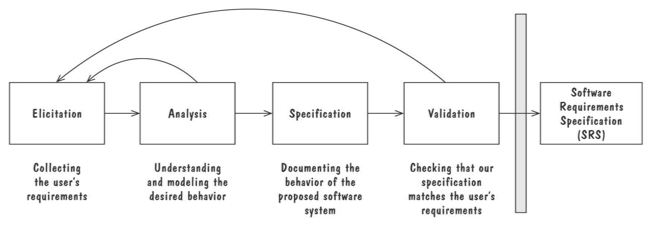
\includegraphics[width=\linewidth]{requirement_process.png}
    \caption{The requirement process}
\end{figure}

In agile method, requirements defined incrementally, essential requirements first,
additional requirements in subsequent releases.

\subsection{Requirements elicitation}

Collecting what the customers (and users) want from the system to be developed.
Need to discuss the requirements with everyone who has a stake in the system.
\newline
Document and review the requirements. \newline
Reach an agreement!

\subsubsection{Stakeholders}

\begin{description}
    \item[Clients] paying for the software to be developed.
    \item[Customers] buying the software after it is developed.
    \item[Users] familiar with the current system and will use the future system.
    \item[Domain experts] familiar with the problem that the software must automate.
    \item[Market researchers] have conducted surveys to determine future trends and potential customer’s needs.
    \item[Lawyers or auditors] familiar with government, safety or legal requirements.
    \item[Software engineers or other technology experts] ensure that the product is technically and economically feasible.
\end{description}

\subsubsection{Means}

\begin{figure}[!ht]
    \centering
    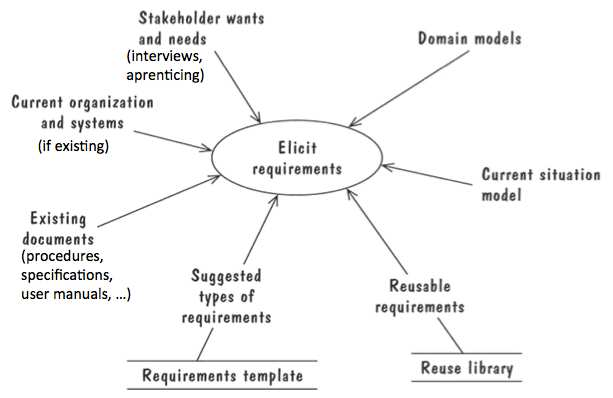
\includegraphics[width=\linewidth]{requirement_process_means.png}
    \caption{Means of the requirements elicitation}
\end{figure}

\todo[inline]{\ldots je ne comprends vraiment pas bien ce que signifie cette image, le paragraphe qui suit
n’est pas nécessaire si ca n’a aucun rapport\ldots}

You have to discuss with the stakeholder in group, to be inspired by other’s ideas. Different
stakeholder have different views, they can lead to inconsistencies. First, prioritize the
requirements and try to reach a compromise. Second, use the view points, in other words
don’t resolve inconsistencies early, keep just separate viewpoints and solve it later when
there is sufficient information.

\subsection{Types of requirements and their desired characteristics}

\subsubsection{Functional requirement:}
It describes a required behaviour in terms of required activities, such as reactions to inputs,
and the state of each entity before and after an activity occurs.

\subsubsection{Quality (or nonfunctional) requirement:}
It describes some required quality characteristic such as fast response time, ease of use,
high reliability, low maintenance costs,\ldots

\subsubsection{Design constraint:}
It is an imposed design decision such as choice of platform or interface components.

\subsubsection{Process constraint:}
It is an imposed restriction on the techniques or resources to be used such as agile methods,
prototypes,\ldots

\subsubsection{Desired qualities of the requirements:}

\begin{description}
    \item[Correct] the requirements conform to the desired understanding.
    \item[Consistent] all requirements can be satisfied simultaneously.
    \item[Unambiguous] requirements have a unique valid interpretation.
    \item[Complete] requirements specify the behaviour under all possible inputs, states and
contexts (externally) and define all terms (internally).
    \item[Feasible] it is possible to realize a system that meets all the requirements.
    \item[Relevant] all requirements correspond to desired or necessary functions or
characteristics.
    \item[Testable] it is possible to demonstrate whether every requirement is met.
    \item[Traceable] all requirements are labelled and organized for easy reference.
\end{description}

\subsection{Nature of requirements definition and specification documents}

\begin{figure}[!ht]
    \centering
    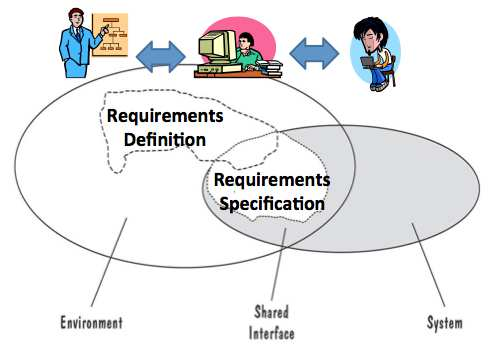
\includegraphics[width=0.6\linewidth]{requirements_documents.png}
    \caption{Two kinds of requirements documents}
\end{figure}

\subsubsection{Software Requirements Definition (SRD):}
Everything the customer wants to achieve, in terms of the environment of the system (i.e.
expressed in the customer’s terms), aimed at a business audience, written by the client and
the requirements analyst/

\subsubsection{Software Requirements Specification (SRS):}

A specification of how the proposed system shall behave, in terms of directly accessible
environment (i.e.\ the boundary of the system), aimed at a technical audience, written by
the requirements analyst for the developers.
Restate the SRD in terms of the system’s interface, with sufficient details, without forcing a
particular design.
